\section{Gradient Boosting}
Der Gradient Boosting Trees (GBT) Algorithmus hat sich in den letzten Jahren als einer der führenden Boosting-Algorithmen etabliert. Charakteristisch für GBT ist die Verwendung von Entscheidungsbäumen als Basis-Lernalgorithmus. Ähnlich wie AdaBoost verfolgt GBT das Prinzip des adaptiven Lernens (\autoref{sec:adaptive_learning}), bei dem jeder nachfolgende Entscheidungsbaum darauf abzielt, die Fehler seines Vorgängers zu korrigieren.

\subsection{Unterschied zu AdaBoost}
Der entscheidende Unterschied zu AdaBoost \ref{sec:adaptive_learning} liegt jedoch in der Art und Weise, wie GBT die Trainingsdaten behandelt. Während AdaBoost die Gewichtung aller Trainingsdaten anpasst, um die Fehler des vorherigen Lerners hervorzuheben, beschränkt sich GBT auf die Redzierung des Restfehlers.
\newline
Obwohl GBT sowohl für Klassifikations- als auch für Regressionsprobleme einsetzbar ist, konzentriert sich diese Arbeit hauptsächlich auf die Anwendung von GBT im Kontext der Regression. Der Grund dafür ist, dass GBT deutlich einfacher verständlich ist in der Art und Weise, wie er kontinuierliche Werte vorhersagt.


\subsection{Die Loss-Funktion \( L \)}
\label{sec:loss_funtion}
Ein wesentlicher Bestandteil des Gradient Boosting Trees Algorithmus ist die Loss-Funktion \( L(y_i,F(x)) \), welche zur Bewertung der Genauigkeit des Modells genutzt wird. Einen zentralen Teil dabei spielen die Residuen. Ein Residuum ist umgangssprachlich ein Fehler, also die Differenz zwischen einem tatsächlichen Datenpunkt \( y_i \) und dem dazu aus dem Modell vorhergesagten Wert \( F(x_i) \).
Im Rahmen von GBT wird häufig der Begriff `Pseudo-Residuen' verwendet. Diese werden in jeder Iteration \( m \) des Algorithmus berechnet und sind definiert als der negative Gradient der Loss-Funktion bezüglich der Modellvorhersage:

\begin{equation}
    \label{eq:residuum_general}
    r_{i,m} = -\frac{\partial L(y_i, F(x_i))}{\partial F(x_i)}\bigg|{F(x)=F{m-1}(x)}
\end{equation}
Im Gegensatz zu einfachen Residuen, welche den Fehler zwischen Vorhersage und tatsächlichem Wert angeben, gibt ein Pseudo-Residuum sowohl die Richtung als auch das Ausmaß der erforderlichen Anpassungen des Modells an. Bei GBT ist das besonders wichtig, da der in jeder Iteration hinzugefügte Entscheidungsbaum speziell darauf trainiert wird, diese Pseudo-Residuen zu minimieren.

\subsubsection{Der Quadratische Fehler (SE)}
Eine häufig genutze Loss-Funktion bei GBT ist der quadratische Fehler (squared error, SE). Gerade für Regressionsprobleme eignet sich die Loss-Funktion SE besonders und ist  definiert als:

\begin{equation}
    L(y_i, F(x_i)) = \frac{1}{2}(y_i - F(x_i))^2 \label{eq:se}
\end{equation}
(Die Konstante 0.5 wird hier o.B.d.A. zur schöneren Auflösung der Ableitung eingefügt.) \\
Setzen wir den SE in die \autoref{eq:residuum_general} für Residuen ein, ergibt sich nach \textcite[S.~346]{Frochte2020}

\begin{equation}
    \label{eq:residuum_se}
    r_{i,m} = y_i-F_{m-1}(x_i)
\end{equation}
Die \autoref{eq:residuum_se} ist zwar nicht mehr so allgemein anwendbar wie \autoref{eq:residuum_general}, ist aber durch die Spezialisierung auf den SE (\autoref{eq:se}) deutlich anschaulicher und leichter zu verstehen.

\subsection{Algorithmus-Struktur und Funktionsweise}
Der folgende Abschnitt erklärt die einzelnen Schritte des GBT-Algorithmus (siehe \autoref{algo:gbt}):

\paragraph{Schritt 1: Initialisierung (Zeile 2)}\label{para:GBT_Initialisierung}
Zu Beginn wird ein Basismodell \( F_0(x) \) erstellt. Häufig, wie auch in dem dargestellten \autoref{algo:gbt}, ist \( F_0(x) \) eine Konstante, die sich aus dem Durchschnitt der Zielwerte \( y\) bildet. Der Hintergrund dafür ist, dass ein solches Basismodell einen guten Ausgangspunkt für die Optimierung bietet, da es bereits eine grundlegende Schätzung der Zielwerte liefert. Diese erste Schätzung wird dann in  folgenden Iterationen verbessert.

\paragraph{Schritt 2: Iterationen (Zeile 3 bis 7)}
Der Hauptteil des Algorithmus ist die Erstellung von Entscheidungsbäumen, welche dann dem Gesamtbaum hinzugefügt werden. Dies passiert über insgesamt \( M \) Iterationen.

\paragraph{Schritt 2.1: Berechnung der Residuen (Zeile 4)}
In jeder Iteration \( m \) werden die Residuen \( r_{m,i} \) für jeden Datenpunkt \( i \) berechnet. Wie in \autoref{sec:loss_funtion} erklärt, zeigen letztere die Abweichung der tatsächlichen Werte \( y_i \) von den Vorhersagen des aktuellen Modells \( F_{m-1}(x_i) \) auf. Die in \autoref{algo:gbt} dafür verwendete Loss-Funktion ist der in SE (\ref{eq:se}.)

\paragraph{Schritt 2.2: Training eines neuen Entscheidungsbaums (Zeile 5)}
\label{para:GBT_training_tree}
In diesem Schritt wird ein neuer Entscheidungsbaum \( h_t \) trainiert, wobei der Fokus nicht auf den ursprünglichen Zielwerten der Trainingsdaten \( (y_i) \), sondern auf den Residuen \( r_{m,i} \) liegt. Jeder Datenpunkt \( (x_i, y_i) \) wird also durch das Paar \( (x_i, r_{m,i}) \) ersetzt, wobei \( r_{m,i} \) das Pseudo-Residuum ist.
\newline
Dies bedeutet konkret, dass der Entscheidungsbaum nicht darauf trainiert wird, die eigentlichen Zieldaten \( y \) direkt vorherzusagen. Stattdessen lernt der Baum, die Fehler des aktuellen Modells, also die Residuen, zu korrigieren. Dadurch das der Baum lediglich die Fehler korrigiert, ergibt es hingegen zu AdaBoost keinen Sinn ihn einzeln zu betrachten. Lediglich im Zusammenhang des Gesamtmodells ist die Hypothese relevant.

\paragraph{Schritt 2.4: Aktualisierung des Modells (Zeile 6)}
Das Modell wird in jedem Schritt verbessert, indem der neue Entscheidungsbaum \( h_m(x) \) zum bisherigen Modell \( F_{t-1}(x) \) mit der Gewichtung \( \alpha \) hinzugefügt wird. Statt als Lernrate einen festen Hyperparameter \( \alpha \) zu benutzen, gibt es auch wie in \textcite[S.~345]{Frochte2020} die Möglichkeit, diesen dynamisch zu berechnen. Meist dann mit \( \gamma \) bezeichnet, ist der Wert meist für jeden Baum unterschiedlich. Für die Suche nach \( \gamma \) kann beispielsweise Linearsuche verwendet werden.
\newline
\newline
Während die Verwendung von \( \alpha \) bedeutet, dass jeder Baum gleichgewichtet ist, lassen sich mit \( \gamma \) feinere und damit auch effizientere Anpassungen am Gesamtmodell machen. Dies ist natürlich aber auch mit einem höheren Rechenaufwand verbunden.

\paragraph{Schritt 3: Ausgabe des finalen Modells (Zeile 8)}
Nach \( M \) Iterationen steht das finale Modell \( F_M(x) \) fest. Es fasst die kumulativen Verbesserungen aller Entscheidungsbäume zusammen und vereint damit alle Verbesserungen zur Anpassung auf die Zieldaten \(y\).

\begin{algorithm}[H]
    \caption[MSE Gradient Tree Boosting]{MSE Gradient Tree Boosting (nach \textcite[S.~346]{Frochte2020})}\label{algo:gbt}
    \begin{algorithmic}[1]
    \State \textbf{Gegeben:} Trainingsdatensatz \( (x_1,y_1), \dots, (x_n,y_n) \)
    \State \textbf{Initialisierung:} Starte mit einem Basismodell \( F_0(x) \), z.B. dem Mittelwert der Labels \( y \)
    \For{\( m = 1, \dots, M \)}
        \State Berechne die Pseudo-Residuen \( r_{i,m} = y_i - F_{m-1}(x_i) \) für alle \( i \)
        \State Trainiere einen Entscheidungsbaum \( h_m \) auf \( (x_i, r_{i,m})_{i=1}^n \)
        \State Führe das Update durch: \( F_m(x) = F_{m-1}(x) + \alpha \cdot h_m(x) \)
    \EndFor
    \State \textbf{Ausgabe:} Das endgültige Modell \( F_M(x) \)
    \end{algorithmic}
\end{algorithm}

\subsection{Beispielanwendung mit Erläuterung}
Um den doch eher abstrakten GBT-\autoref{algo:gbt} zu veranschaulichen, wird im folgenden die Funktionsweise anhand des Beispiels in \autoref{fig:gbt-example} beschrieben.
\newline
Die Abbildungen sowie die verwendeten Daten entstammen einem eigenen Programm, welches mithilfe von SKLearn in Python erstellt wurde. Die genaue Implementierung ist auf  \textbf{\href{https://github.com/CodeLtDave/Boosting-Algorithms-ML-Seminararbeit/blob/main/python-env/GBT-Example.ipynb}{meinem GitHub Repo}} zu finden. Wir betrachten den folgenden synthetischen Datensatz als gegeben:

\begin{verbatim}
X, y = make_regression(n_samples=100, n_features=1, noise=10, random_state=42)
X_sorted, X_indices = np.sort(X, axis=0), np.argsort(X, axis=0)
\end{verbatim}
Wie im oberen Bild der \autoref{fig:gbt-example} zu erkennen ist, wird im Schritt der Initialisierung zunächst das Basismodell aus dem Durchschnitt der Zielwerte gebildet. Wie zu erwarten, hat das Basismodell keine wirkliche Aussage über die Zieldaten mit einem MSE von 1690.
\newline
\newline
In der ersten Iteration wird dann eine erste Vorhersage auf die Daten getroffen. Für diese Iteration stehen natürlich noch keine Residuen des Vorgängermodells zur Verfügung, weshalb sich die Punkte der Daten und Residuen decken. Schon nach einer Iteration nimmt die Vorhersage die ungefähre Form der Daten an. Alleine in diesem Schritt kann der MSE um das 5-fache reduziert werden.
\newline
Hier lässt sich zum ersten mal das Prinzip der Residuen veranschaulichen. Nehmen wir als Beispiel den einzelnen Datenpunkt in der unteren linken Ecke. Die Gesamtvorhersage der ersten Iteration hat eine Abweichung von ca. 80. Genau diese Abweichung von ca. 80 spiegelt sich dann für die zweite Iteration bei dem Residuum in der unteren linken Ecke wieder. In der zugehörigen Baumvorhersage lässt sich auch erkennen, dass sie deutlich besser auf die Residuen passt als die Ursprungsdaten. Trotzdem lässt sich in diesem Schritt der MSE fast halbieren. Dies veranschaulicht die Argumentation aus \hyperref[para:GBT_training_tree]{Schritt 2.2}.
\newline
\newline
Nach der dritten Iteration entspricht die Gesamtvorhersage ziemlich genau den Daten mit einem verbleibenden MSE von 89. Neben der schrittweiten Verbesserung des Modells lässt sich eine weitere Beobachtung treffen: In jeder Iteration nähern sich die Residuen der X-Achse an. Nach einer unbekannten Iteration von Schritten ist davon auszugehen, dass, wenn die Gesamthypothese die Daten perfekt abbildet, sich alle Residuen auf der X-Achse befinden.

\subsection{ Weiterentwicklung XGBoost}
Eine der am häufigsten in der Praxis zitierten Ausprägungen von GBT ist dessen Weiterentwicklung XGBoost. Hierbei wurden eine Reihe von Verbesserungen und Beschleunigungen vorgenommen.
\newline
Unter anderem verwendet XGBoost die Loss-Funktion direkt statt deren negativen Gradienten sowie führt sogenannte Regularisierungsterme ein, um Überanpassung des Lernens an die Trainingsdaten (Overfitting) zu vermeiden.
XGBoost oder andere Weiterentwicklungen werden jedoch hier nicht weiter betrachtet.

\begin{figure}[h]
    \centering
    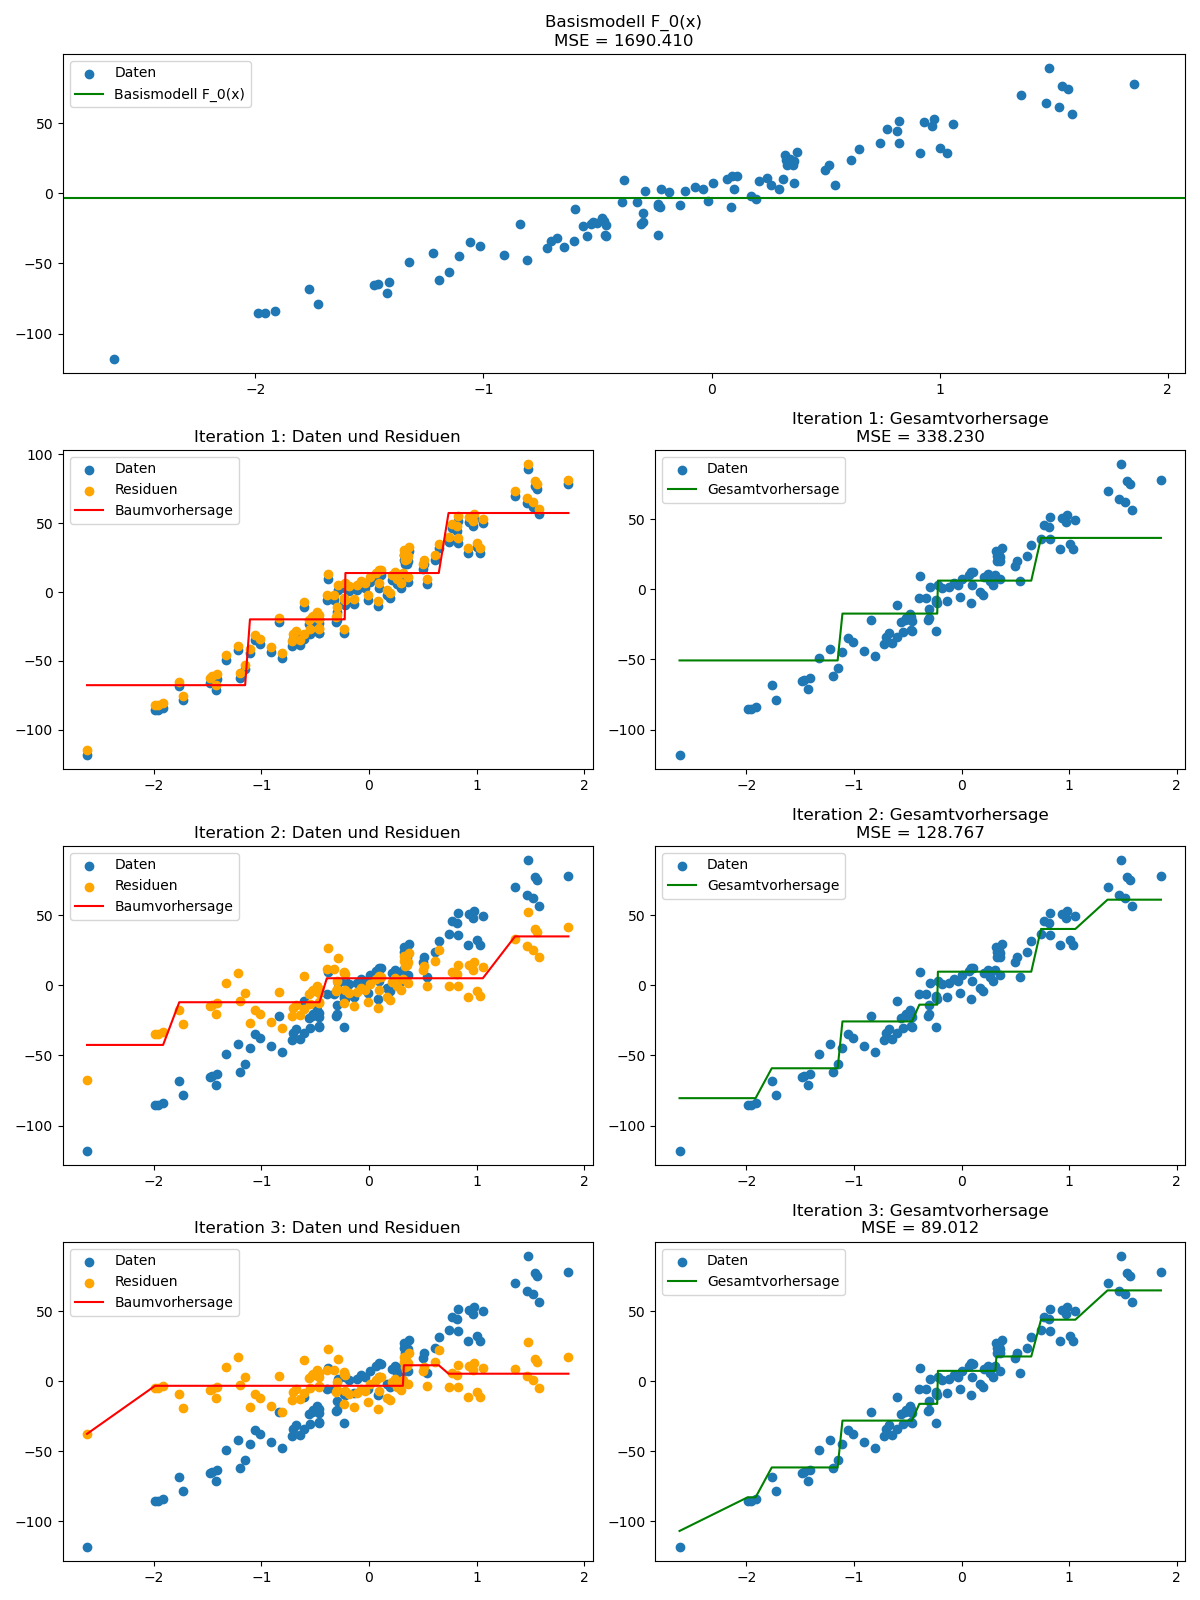
\includegraphics[width=0.8\textwidth]{Images/GBT_Example.png}
    \caption[Visualisierung des Gradient Boosting Trees Algorithmus]{Visualisierung des Gradient Boosting Trees Algorithmus.}
    \label{fig:gbt-example}
\end{figure}